%%%%%%%%%%%%%%%%%%%%%%%%%%%%%%%%%%%%%%%%%%%%%%%%%%%%%%%%%%%%%%%%%%%%
% Experimentación con algoritmo inicialización aprendida DE PESOS
%%%%%%%%%%%%%%%%%%%%%%%%%%%%%%%%%%%%%%%%%%%%%%%%%%%%%%%%%%%%%%%%%%%%

En la siguiente sección trataremos sobre la bondad del algoritmo expuesto

\section{Contraste de hipótesis con inicialización aleatoria} 
\label{ch07:experimento-1} 

Las preguntas a resolver son ¿mejora nuestro algoritmo? ¿Cuánto mejora?

La primera observación  es que como
hemos observado en el modelado de una red neuronal 
en la sección \ref{ch05:construction-evaluation-nnnn}
una red neuronal depende de varios parámetros:
la dimensión de entrada $d$, el número de neuronas en la capa oculta $n$, la dimensión de salida $s$ 
y la funciones de activación de cada neurona.  

Por simplicidad fijaremos una función de activación. 


\subsection{Descripción experimento}

El experimento consta de los siguientes pasos: 

\begin{enumerate}
% Paso 0: Selección de data sets 
\item Dado un conjunto de datos de entrenamiento $\D$  se separará el conjunto en:
\begin{itemize}
    \item $\D_i$ \textbf{Conjunto de 
    datos de entrenamiento e inicialización.} Debe de ser mayor que 
    $n$ y lo suficientemente grande para que el algoritmo diseñado funcione correctamente. 

    \item $\D_t$ \textbf{Conjunto de 
    datos de test.} Se utilizarán para el cálculo del error. 
\end{itemize} 

En particular hemos utilizado el conjunto de datos \href{https://archive.ics.uci.edu/ml/datasets/Airfoil+Self-Noise
    }{
        Airfoil Self-Noise} obtenido del repositorio de datos libres para aprendizaje automático \href{https://archive.ics.uci.edu/ml/datasets.php}{UCI}. 
El conjunto elegido se corresponde a un problema de regresión con $1503$ instancias y $6$ atributos. 
Para la implementación realizada podría utilizarse cualquier otra que provenga de un problema de regresión. 

Notemos que $d$ viene determinado por el número de atributos, 
$s$ será uno ya que estamos frente a un problema 
de regresión de variable real y $n$ vendrá dado como $n = \lfloor \alpha |\mathcal{D}_i| \rfloor$ con $\alpha \in (0,1)$; concretamente, en virtud de la observaciones mostradas en la 
sección \ref{section:inicializar_pesos} de que la probabilidad de 
que un dato no pueda ser utilizado para el algoritmo es nula; 
suponer que el $90\%$ de los datos sí serán válidos es una 
estimación lo suficientemente precavida como para que el algoritmo 
no \textit{falle}, es decir haremos    $\alpha = 0.9$. 

% Paso 1: Construcción 
\item Fijados $n, d$ y $s$ se generarán dos redes neuronales: 

\begin{itemize}
    \item Una inicializada de manera aleatoria con valores dentro de un rango de valores. 
    
    \item  Otra inicializada con nuestro algoritmo, se medirá el $t_i$ tiempo y el error $\varepsilon_i$ en  $\D_t$. 
\end{itemize}

% Paso 2: Evaluación del error
\item Con los datos de entrenamiento $D_i$ y el algoritmo de 
aprendizaje de \textit{backpropagation} se entrenará la red 
neuronal inicializada aleatoriamente hasta que iguale o sea menor que  el 
error del algoritmo de inicialización aprendida $\varepsilon_i$. 

Puesto que puede darse el caso de 
quedar estancados en un mínimo local superior al error encontrado con el algoritmo de inicialización aprendida $\varepsilon_i$ o que oscile entorno a un 
mínimo si el $\eta$ no es lo suficientemente pequeño (ver 
propiedades del gradiente descendente \ref{ch05:gradiente-descentente}); se ha añadido también como criterio de parada el que el error del algoritmo de \textit{backpropagation}
se estanque o empeore durante 5 \footnote{El valor de 5 
iteraciones consecutivas es una heurística observada en 
ejecuciones anteriores y dependiente de $\eta$ y del problema.
Pude observar la traza de de ejecución si ejecuta el experimento.} 
iteraciones consecutivas. 

Durante el experimento se medirá el tiempo que necesita hasta su fin $t_b$ y el error en 
entrenamiento y test. 

Los tiempos $t_i$ y $t_b$ serán los que compararemos con el test de hipótesis. 
\end{enumerate}

Los pasos 2 y 3 se repetirán tantas veces como 
muestras se desee tomar. 

\subsection{Contraste de hipótesis}

Se desea comparar si las diferencias en los tiempos observados efectivamente son notables: 

Para ello se realizará un test de Wilcoxon, con las siguientes hipótesis

\begin{itemize}
    \item $H_0$: La mediana de la diferencia de tiempos  $t_i$ y $t_b$ de cada par de muestras es cero. 
    \item $H_a$: La mediana de las diferencia de tiempos  $t_i$ y $t_b$ entre cada par de muestras es diferente de cero. 
\end{itemize}

La utilidad de este test es que si rechaza la hipótesis nula sabremos que con un $95 \%$ de certeza tendrán medianas diferentes, es decir, \textbf{existe una 
diferencia en los errores}. En caso de que no se rechace no podremos afirmar nada.
Puede encontrar la implementación en el repositorio del
 proyecto \footnote{En el directorio de experimentos 
 de \url{https://github.com/BlancaCC/TFG-Estudio-de-las-redes-neuronales}.}.

\subsection{Requisitos técnicos}  

A la vista de todo el proceso descrito surgen las siguientes necesidades técnicas que deberemos de implementar:  

\subsubsection{Lectura y tratamiento de los datos}

Se necesita ser capaces de leer los datos desde los ficheros descargados, es decir, ser capaces de transformar el formato \textit{.dat} en un \textit{.csv}. 
Además, es necesario un tratamiento previo de los datos: 
\begin{itemize}
    \item Comprobación de que no hay valores nulos o perdidos. 
    \item Normalización de los datos. 
\end{itemize}


\subsubsection{Capacidad de crear una red neuronal aleatoria}  

Deberá de crearse una red neuronal con entradas dentro de un rango $[a,b]$ con $a < b$ reales,
que tenga una entrada de tamaño $d$,
$n$ neuronas en la capa oculta y
una dimensión de salida $d$.

\subsubsection{Implementación del algoritmo de inicialización aprendida}

Deberá implementarse el algoritmo  \ref{algo:algoritmo-iniciar-pesos} con todos los requisitos y atributos que ahí se describe.  

\subsubsection{Función para medir el error}

Deberá implementarse una función para medir el
 error, puesto que nos hayamos frente a un problema de regresión utilizaremos el error cuadrático medio. 

\subsubsection{Forma de evaluar las redes neuronales}  

Dados una red neuronal, una función de evaluación y un vector de atributos de dimensiones adecuadas a la red neuronal debe ser capaz de aplicar el algoritmo de \textit{forward propagation} descrito en \ref{algoritmo:evaluar red neuronal}.

\subsubsection{Implementación del aprendizaje de una red neuronal} 
% Nota en el margen sobre la derivada
\marginpar{\maginLetterSize
    \iconoAclaraciones \textcolor{dark_green}{     
        \textbf{
            Qué es una derivada débil.
        }
    }
    Es una generalización de las derivadas para funciones del espacio $L_p$, esto nos permite
    definir derivadas aunque no lo sea en algunos puntos (recodemos que demostremos el teorema de aproximación universal para estos espacios en la sección \ref{ch04:espacios-Lp}).   
}
Se implementará el algoritmo propio de aprendizaje basado en \textit{backpropagation} y ya optimizado 
que describimos en los algoritmos \ref{algoritmo:gradiente-descendente} y \ref{algoritmo:calculo-gradiente}.
Cabe destacar que para este algoritmo es necesario usar la derivada de las funciones de las funciones de activación. Se ha implementado la derivada débil de ellas. Además se ha seguido el mismo criterio de diseño que ya se tuvo con las funciones de activación en la sección \ref{ch06:activation-function-implementation}.

\subsubsection{Implementación del experimento} 
Deberá implementarse una función que realice el 
experimento tal cual hemos descrito en \ref{ch07:experimento-1}.

\subsection{Resultados obtenidos}

Concretamente de el experimentos se ha realizado con 
una partición del conjunto de datos $\frac{3}{4}|\mathcal{D}|$ para entrenamiento entrenamiento 
y el resto de test. Se ha repetido además $15$ veces (por tratarse de un número conveniente de muestras para el Test de los signos de Wilcoxon como vimos en la sección \ref{ch06:test-hipotesis-propiedades} donde se usó por primera vez). 

Durante cada iteración los datos del conjunto han sido desordenados y el tiempo medido ha sido estrictamente el de creación y aprendizaje de la red neuronal. 

Puede consultar los resultados obtenidos en 
\href{https://github.com/BlancaCC/TFG-Estudio-de-las-redes-neuronales/tree/main/Experimentos/inicializacion-pesos-red-neuronal/resultados/2_air_self_noise}{la carpeta de experimentos de air self noise} 
de nuestro repositorio, es más para obtener
 una información detallada del mismo ejecute 
 los experimentos y observe la información que van mostrando. 


De donde se tiene que para nuestro algoritmo de inicialización aprendida el tiempo medio de ejecución es de 
\begin{equation}
    0,044 \pm 0,064 \text{ segundos, }
\end{equation}
mientras que para la inicialización aleatoria y aprendizaje con el método de 
\textit{backpropagation} es de 
\begin{equation}
    5,284 \pm 0,407   \text{ segundos}.
\end{equation}

Además el test de los signos de Wilcoxon ha rechazado la hipótesis nula
con un $95\%$ de confianza,
por lo que podemos afirmar que efectivamente la diferencia de tiempos es significativa. 

El gráfico de caja bigote con los tiempos es el siguiente: 

\begin{figure}[H]
    \centering
     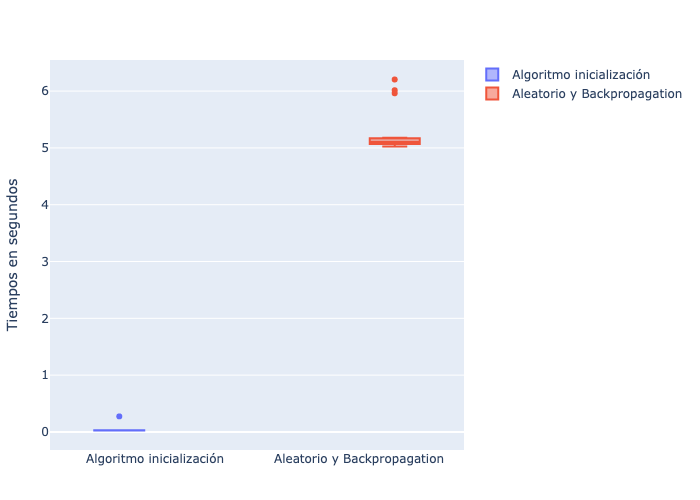
\includegraphics[width=0.8\textwidth]{7-algoritmo-inicializar-pesos/experimento/grafico-bigotes-tiempo.png}
     \caption{Gráfico de caja y bigotes del tiempo requerido por el algoritmo de inicialización aprendida de pesos y el de \textit{backpropagation}.}
\end{figure}
Debemos ser cautos antes de afirmar que tal relación entre los tiempos es el índice de mejora. Puesto que antes debe de conocerse el motivo por el que se detuvo el algoritmo de \textit{backpropagation}; para ello se estudiará la distribución de los errores en entrenamiento. 

\begin{figure}[H]
    \centering
     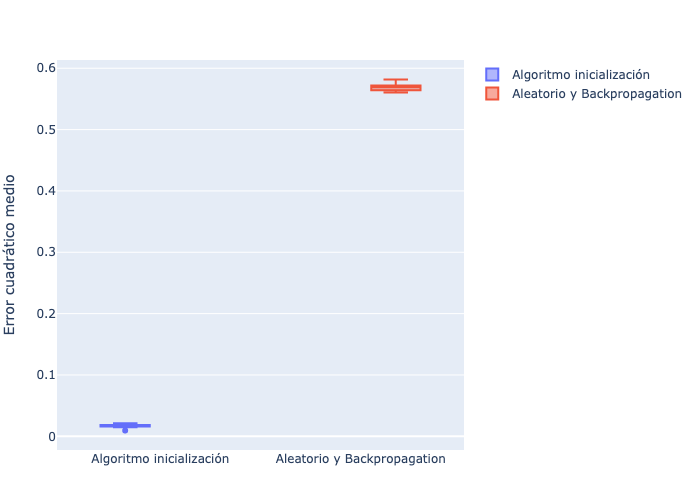
\includegraphics[width=0.8\textwidth]{7-algoritmo-inicializar-pesos/experimento/grafico-bigotes-error_entrenamiento.png}
     \caption{Gráfico de caja y bigotes del \textbf{error en entrenamiento tras finalizar } el algoritmo de inicialización aprendida de pesos y el de \textit{backpropagation}.}
     \label{img07:error-entrenamiento}
\end{figure}

En promedio el error cuadrático medio dentro del entrenamiento conseguido con nuestro algoritmo es 
\begin{equation}
    0,017 \pm 0,003;
\end{equation}
mientras que el de inicialización aleatoria y \textit{backpropagation} es de 
\begin{equation}
    0,569 \pm 0,006. 
\end{equation}
Si además se observa la traza obtenida durante la ejecución (ver repositorio), 
no tarda uno en percatarse de que en la mayoría de las muestras, la parada del algoritmo de
\textit{backpropagation} se está produciendo al \textit{estancarse} el error 
en un mínimo local. 

Esta situación si bien nos previene de poder explicitar un coeficiente de mejora 
entre el algoritmo de inicialización aprendida y \textit{backpropagation} desde 
una red neuronal inicializada aleatoriamente, pone de manifiesto su gran potencial de aprendizaje. 
Es por tanto interesante  comparar el error cuadrático medio obtenido en los datos de test, ya que nos dará una estimación verdadera de la bondad del método.  

El error cuadrático medio de ambos métodos en test es el siguiente: 
\begin{figure}[H]
    \centering
     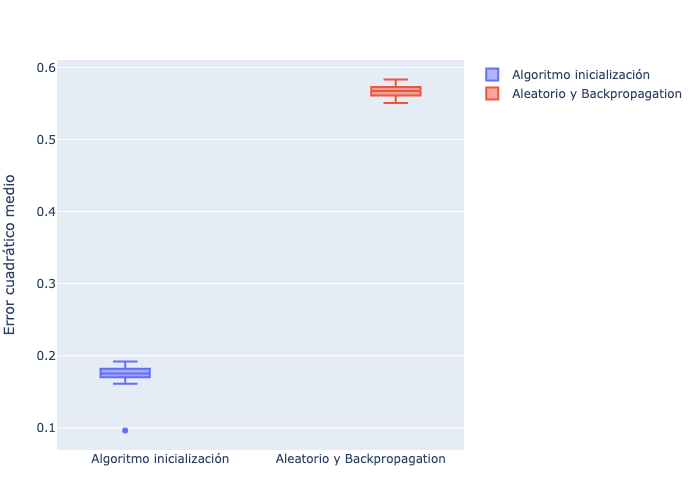
\includegraphics[width=0.8\textwidth]{7-algoritmo-inicializar-pesos/experimento/grafico-bigotes-error_test.png}
     \caption{Gráfico de caja y bigotes del \textbf{error cuadrático medio en test } el algoritmo de inicialización aprendida de pesos y el de \textit{backpropagation}.}
     \label{img07:error-test}
\end{figure}

donde ahora el promedio para nuestro algoritmo de inicialización aprendida es de un error de
\begin{equation}
    0,171 \pm 0,022;
\end{equation}

% Nota sobre sobreajuste 
\marginpar{\maginLetterSize
    \iconoAclaraciones \textcolor{dark_green}{     
        \textbf{
            ¿Qué significa que un modelos está sobreajustado o sobreentrenado?
        }
    }
    En aprendizaje automático un modelo se dice sobreentrenado o sobreajustado 
    cuando ha \textit{aprendido} características 
    propias de los datos de entrenamiento que 
    no son válidas para el problema general. 
    Este efecto produce que se tengan resultados en 
    entrenamiento \textit{considerablemente} mejores que en test.   
}
% fin de la nota
mientras que el de inicialización aleatoria y \textit{backpropagation} es de 
\begin{equation}
    0,567 \pm 0,009.
\end{equation}


A diferencia del error en test obtenido con \textit{backpropagation}, el de nuestro algoritmo
 ha superado al de entrenamiento, lo que indica un sobreajuste 
del modelo a los datos de entrenamiento. Esto es totalmente de esperar por 
cómo se construye la inicialización de pesos. Sin embargo, a pesar del sobreajuste, el resultado sigue siendo mejor tanto en precisión como en tiempo que el de aprendizaje usando \textit{backpropagation}.  


\section{Observaciones y conclusiones sobre el algoritmo de inicialización aprendida de pesos}


Cabe destacar que si bien el algoritmo se ha diseñado para nuestro 
modelo de red neuronal, la idea se puede extender al resto de modelos 
existentes; para ello bastaría seguir la
demostración y plantear el sistema de ecuaciones adecuado que se 
utilizan en la línea 4 del algoritmo \ref{algo:algoritmo-iniciar-pesos}.

Por otro lado, en nuestro caso concreto, el algoritmo
 de inicialización aprendida ha presentado 
 mejores resultados en precisión y tiempo que la 
 alternativa, esta simultaneidad en los 
 beneficios evita cuantificarlos; ya que para 
 tener un coeficiente de mejora o tiempo debería de fijarse un parámetro (las mismas condiciones de observación) y comparar el otro. 

 Como mostramos por el experimento no ha sido 
 posible fijar el error de estudio, ya que 
 \textit{backpropagation} no ha sido capaz de minimizar la red inicializada aleatoriamente 
 hasta tal error. 

 Por otro lado nuestro algoritmo al no ser iterativo tampoco ha podido adaptarse al de 
 \textit{backpropagation}. 

 Si razonáramos fijando el error, la comparación tampoco es posible, ya que si se observan los tiempo de la traza de ejecución (ver experimento en el repositorio), una sola ejecución de nuestro
 algoritmo ya es más rápida que una iteración de 
 \textit{backpropagation}. 

Para futuros trabajos se podría cuantificar la mejora, para ello
proponemos relajar restricciones de \text{backpropagation} con el fin de 
reducir su tiempo de ejecución y así poder compararlos.
 Proponemos para 
ello reducir el tamaño del conjunto de entrenamiento en cada iteración. De esta forma se podría obtener un tiempo por iteración que sea 
divisor del que emplee el algoritmo de inicialización aprendida 
y de esta manera sí poder fijar un tiempo común con el comparar el error. 
\newpage

